% 
\newpage\section{Opis dziedziny przedmiotowej pracy}\label{sec:dziedzina}
\subsection{Pojęcia i definicje}
W dokumencie tym posługiwać się będziemy następującymi pojęciami:

Klucz dostępowy - jest to klucz publiczny z pary kluczy prywartny publiczny. Używany jest on do odszyfrowania wiadomości wysłanej z aplikacji mobilnej do urządzenia sterujacego.

Klucz szyfrujący jest to klucz prywatny wygenerowany podczas tworzenia pary kluczy publiczny prywatny. Używane jest on do szyfrowania wiadomości wysyłanej z aplikacji mobilnej do urządzenia sterującego

para kluczy szyfrujących- jest to para kluczy (prywatny oraz publiczny) generowanych podczas rejestracji oraz wymiany klucza dostepowego.

Inteligentny zamek - system obsługujący otwieranie elektrozamka bądz serwomechanizmu.
\subsection{Stan wiedzy}
Przed przystąpieniem do projektu zrobiliśmy porównanie systemów zbliżonych do naszego który na dany moment istniały. I tak doszliśmy do wniosku że wszystkie systemy inteligentnych zamków wykonane przez firmy takie jak Gerda Lock czy Danalock zostały wykonane typowo dla użytku domowego a nie tak jak nasz projekt inżynierski który jest przeznaczony do zarządzania w budynkach o wielu pomieszczeniach z różnym stopniem dostępu. Opis wraz z porównaniem poszcególnych systemów znajduje się w tabelach poniżej.


	Tabela \ref{tab:porownanie1} zawiera porównanie firm pod względem otwierania zamka
	\begin{longtable}[!ht]{|p{4cm}|p{1,5cm}|p{1,5cm}|p{1,5cm}|p{1,5cm}|} 
		\caption{Tabela porównania otwierania zamków}
		\label{tab:porownanie1}\\
		\hline	
		 & NOKI & August & DanaLock & Gerda Lock  \\	\hline
		 zarządzanie wieloma zamkami z jednej aplikacji
		 & brak & tak & brak & brak \\	\hline
		otwieranie zamka przy pomocy strony WWW
		& brak & brak & tak & brak \\	\hline
		inne sposoby otwarcia zamka niż aplikacja
		& brak informacji& brak informacji & brak & tak \\	\hline
		automatyczne zamykanie zamka
		& brak informacji& tak & tak & tak   \\	\hline
		tryb otwierania zamka automatycznie
		& tak& brak & tak & tak \\	\hline	
		tryb otwierania zamka po zezwoleniu przyciskiem
		& brak & tak & tak & tak \\		\hline
	\end{longtable}


 
 	Tabela \ref{tab:porownanie2} zawiera porównanie firm pod względem zasilania i montażu
 \begin{longtable}[!ht]{|p{4cm}|p{1,5cm}|p{1,5cm}|p{1,5cm}|p{1,5cm}|} 
 	\caption{Tabela porównania zasialania i montażu}
 	\label{tab:porownanie2}\\
 	\hline	
 	& NOKI & August & DanaLock & Gerda Lock  \\	\hline
 	zasilanie zewnętrzne (z sieci)	
 	& brak & brak & brak & brak \\	\hline
	 zasilanie bateryjne (podstawowe/ awaryjne)	
	 & podstawowe & podstawowe & podstawowe & podstawowoe \\	\hline
 	sposób montażu	
 	& nakłądka na zamek & nakłądka na zamek & nakłądka na zamek & nakłądka na zamek \\	\hline
 \end{longtable}
 



Tabela \ref{tab:porownanie3} zawiera porównanie firm pod względem dziennika zdarzeń oraz powiadomień
\begin{longtable}[!ht]{|p{4cm}|p{1,5cm}|p{1,5cm}|p{1,5cm}|p{1,5cm}|} 
	\caption{Tabela porównania zasialania i montażu}
	\label{tab:porownanie3}\\
	\hline	
	& NOKI & August & DanaLock & Gerda Lock  \\	\hline
	podgląd kto otworzył	
	& brak informacji & brak & brak & tak \\	\hline
	
	
	powiadomienie o otwarciu drzwi (ogólnie i przez daną osobę)
	& brak & brak & brak & tak \\	\hline
	
	
	powiadomienie o nieautoryzowanych próbach otwarcia
	& tak & brak & brak & tak \\	\hline
\end{longtable}





\subsection{Stan pracy wykonany w ramach zajęć \newline przedmiotowych} 
W ramach zajęć projektowych oraz laboratoryjnych o nazwe Projekt Zespołowy prowadzonych z mgr. Michałem Apolinarskim oraz dr Ewą Idzikowską zostały wykonane następujace fragmenty systemu:
	Aplikacja mobilna została wykonana dla wersji andorida minimum 4.4 KitKat w stopniu umożliwiającym takie funkcjonalnośći jak:
	\begin{itemize}
		\item Logowanie
		\item Rejestracja
		\item Rejestracja wraz z tworzeniem pary kluczy dostępowych publiczny prywatny
		\item Generowanie nowego certyfikatu
		\item Pobieranie certyfikatów z serwera
		\item Zarządznanie certyfikatami użytkownika
		\item Zarządzanie prośbami o rejestracje
		\item Wnioskowanie o certyfikat nowy
	\end{itemize}
		Dodatkowo zostało napisane api do obsługi połączenia bluetooth oraz w każdym widoku któy korzystał z połaczenia z serwerem były napisane fragmenty kodu. Funkcje te oraz kod zostały napisane bez uwzględnienia wzorców architektoniczncych (wszystko co dotyczyło danego widoku było w jednej klasie), posiadały szereg błędów powodujaćych niestabilne działąnie systemu oraz posiadały metody z systemu android które były określane przez środowisko android stuido jako "deprecated" co mogło przy nowszych wersjach androida powodować wadliwe działanie systemu. Z racji pisania pod wersje systemu android 4.4 wygląd różni się od tego który został zaimplementowany w pracy inżynierskiej. Ponieżej przedstawiono wygląd aplikacji w stanie początkowym(????).
		 
	
	
    Aplikacja serwerowa posiadałą następujące rest api
    \begin{itemize}
    	\item api służące do pobierania certyfikatu
    	\item api służące do informowania o statusie certyfikatu
    	\item api służące do logowania użytkownika
    	\item api służące do rejstracji uzytkownika
    	\item api służące do wylogowania użytkownika
    	\item api służące do pobrania wszystkich certyfikatów użytkowników
    	\item api służące do pobrania listy wszystkich zamków
    	\item api służące do pobrania listy wszystkich uzytkownikóW systemu
    	\item api służące do zmiany hasła
    	\item api służące do pobrania histori użycia zamków
    	\item api służące do pobrania listy oczekujących certyfikatów
    	\item api służące do pobrania listy oczekujących użytkowników na zarejestrowanie
    	\item api służące do generowania nowego certyfikatu
    	\item api służące do określenia decyzji administratorwa w stosunku do danego oczekującego certyfikatu
    	\item api służące do określenia decyzji administratorwa w stosunku do danego oczekującego użytkownika na zarejestrowanie 
    \end{itemize}   
	Wszystkei te api zwracały odpowiednio albo odpowiednie dane albo wartość Invalid. Ponadto posiadały szereg niedopatrzeń powodujących wadliwe działanie systemu w szcególnych przypadkach. 
	
	Urządzenie sterujące zamkiem
	???????????????????????????????????????????????????????????????????????????????
	
	Baza danych została wykonana w następujaćy sposób: 
	
		\begin{figure}[!h]
		\centering
		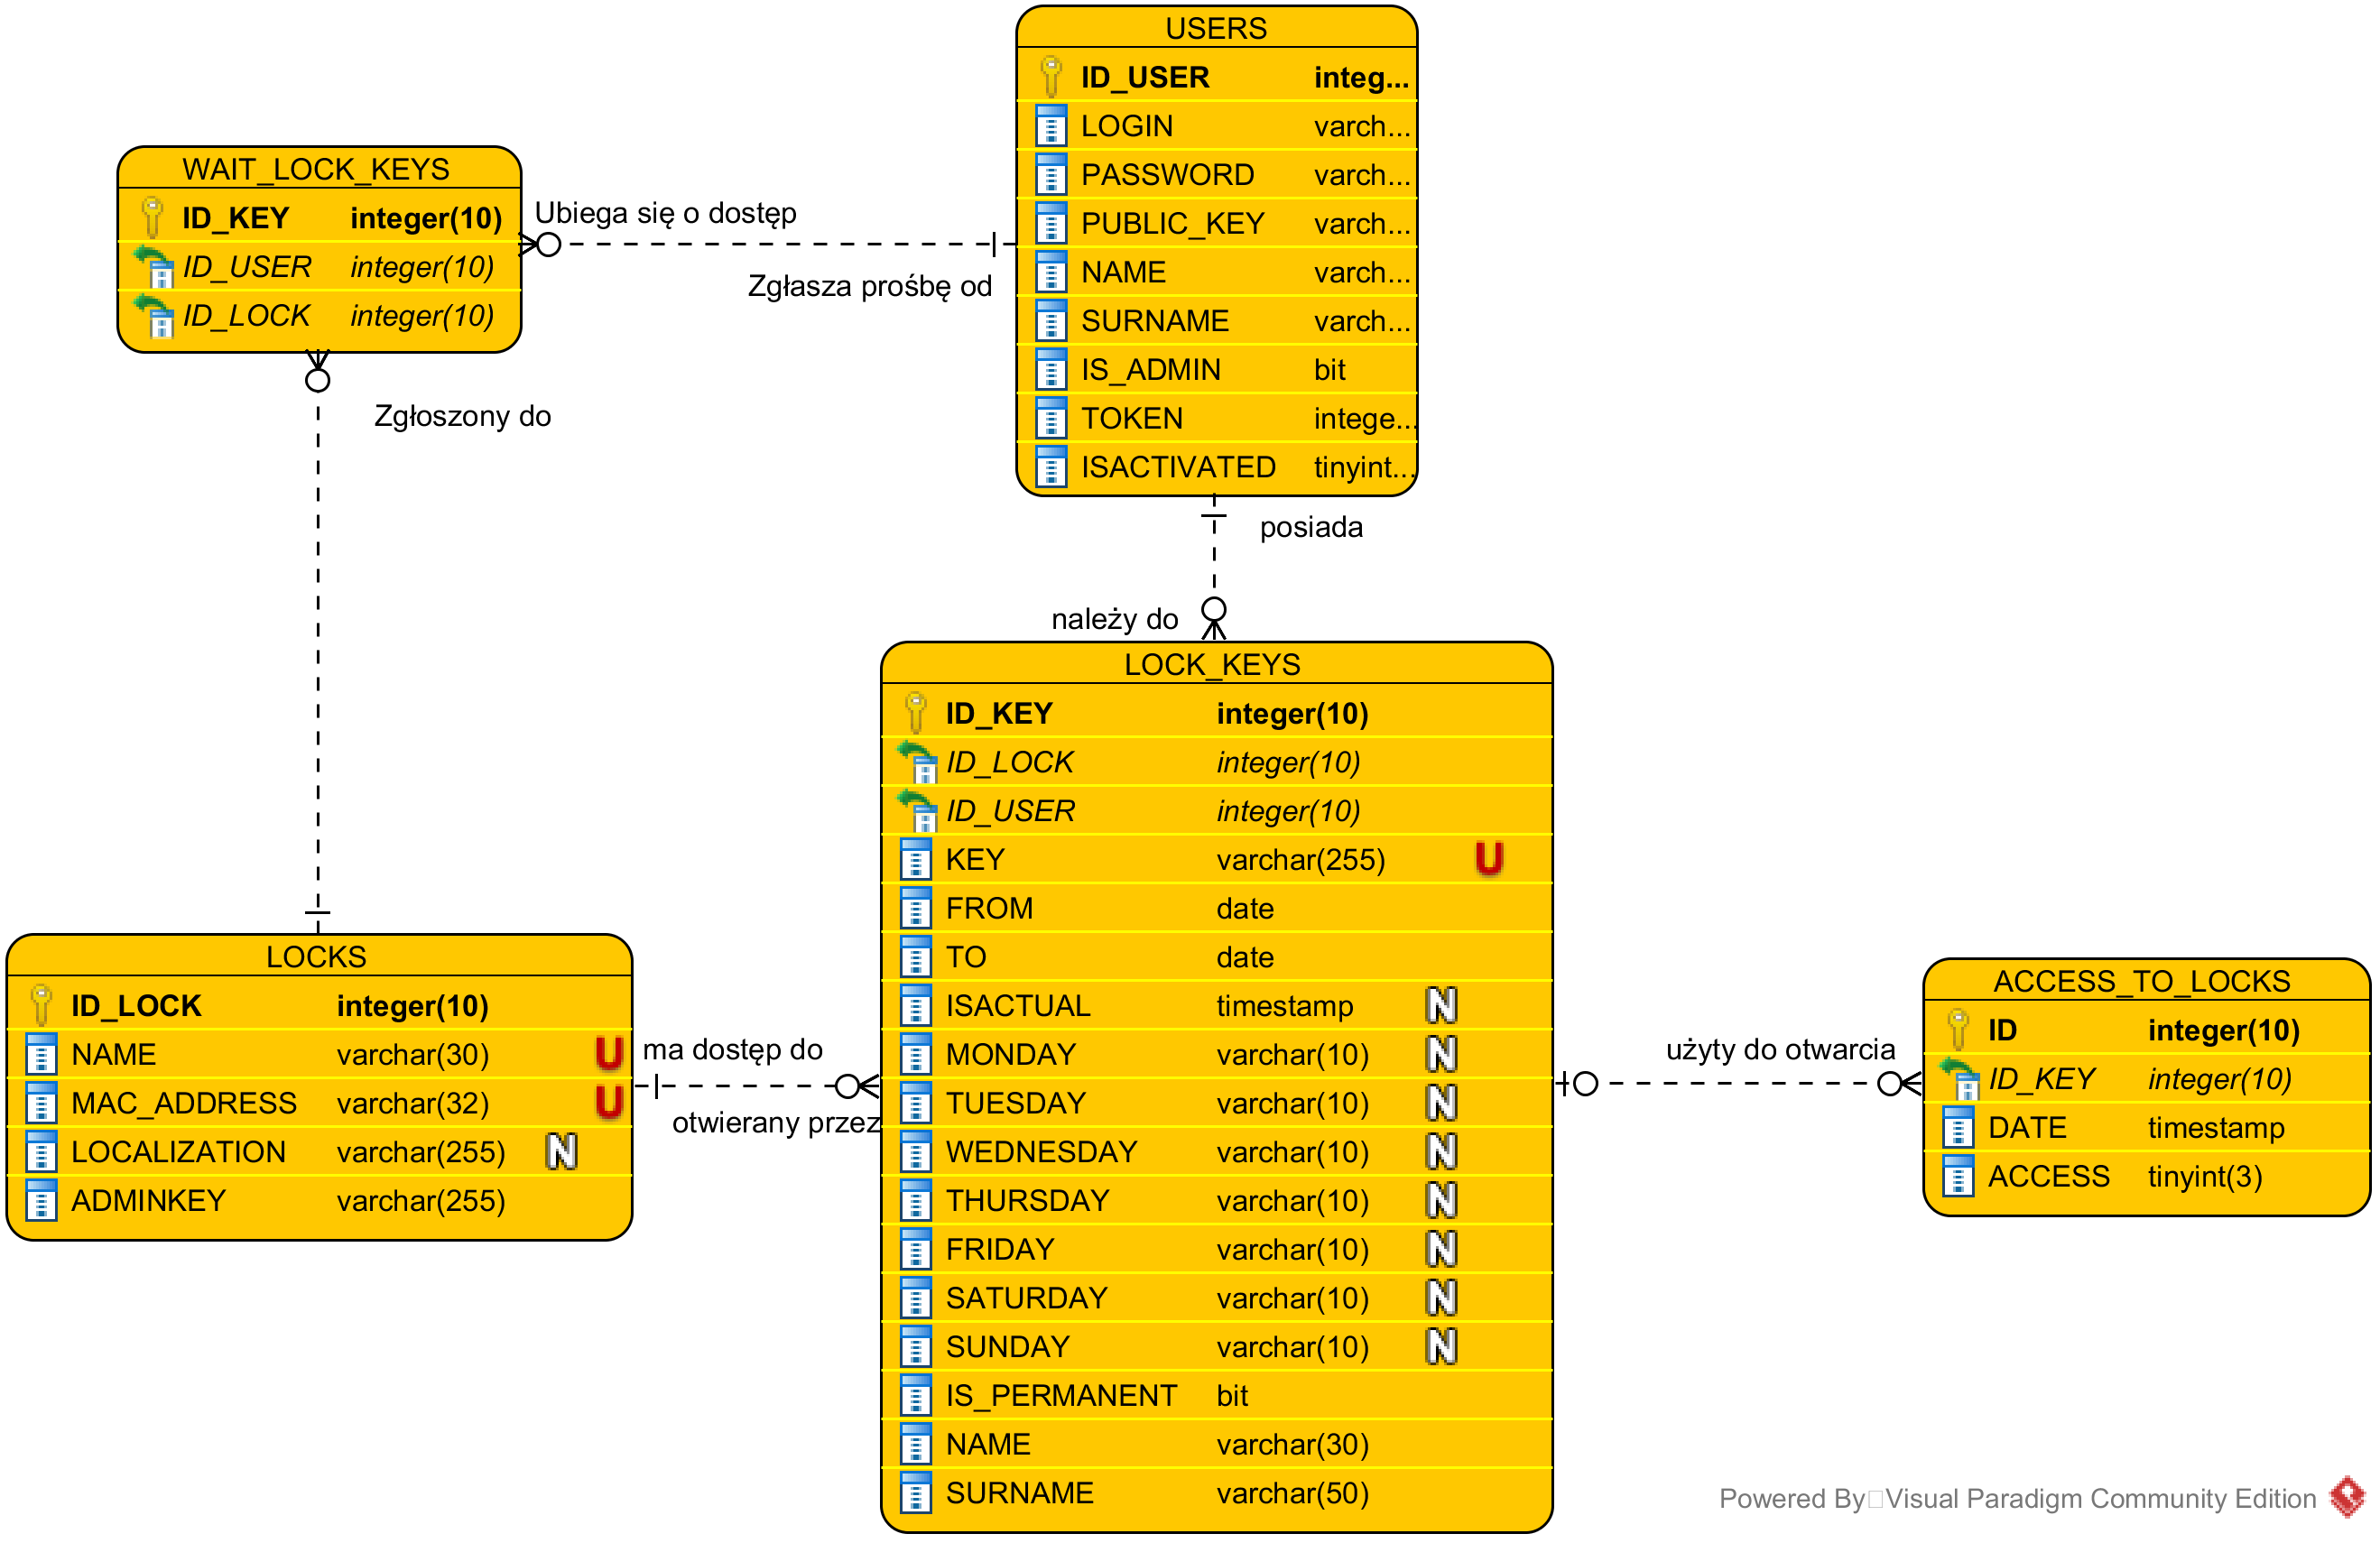
\includegraphics[width=16cm]{Obrazy/Diagram_relacjOld.png}
		\label{diagram:diagram relacji}
	\end{figure}

	W ramach przedmiotu ochrona danych zostały zaimplementowane w systemie fragmenty PKI takie jak:
	   \begin{itemize}
	   	\item Certyfikat klucza dostępowego
	   	\item  generowanei nowego Certyfikatu uzytkownika
	   	\item blokowanie uzytkownika systemu
	   \end{itemize}
	 Funkcje te zostały napisane zarówno po stronie aplikacji mobilnej jak i aplikacji serwerowej. Ponadto po stronie androida został opracowany sposób przechowywania klucza prywatnego w formie zaszyfrowanego pliku hasłem uzytkownika.
